% ============================ 附录 ============================
\section{50 维感官维度的 Top-3 关键化合物全表}

正文表~\ref{tab:top3} 只摘录了 11 个代表维度，完整结果见表~\ref{tab:top3full}。
其中括号内数字为该化合物在 200 次 bootstrap 重采样中的入选频率
（口径见 \S6.3：重采样后 Spearman 绝对秩相关进入前 10 即计入选）。

\begin{table}[H]
\centering
\caption{50 个感官维度的 Top-3 关键化合物全表（按规范化学名给出，括号内为 bootstrap 入选频率）}
\label{tab:top3full}
\scriptsize
\begin{fittable}
\begin{tabular}{@{}llllr@{}}
\toprule
感官维度 & Top-1 & Top-2 & Top-3 & 方法 $J$ \\
\midrule
麦芽香-总体 & beta.phellandrene（0.71） & Furfural（0.27） & Octyl acetate（0.12） & 0.15 \\
麦芽香-谷物 & X5.methylfurfural（0.14） & Isoborneol（0.65） & Furfural（0.34） & 0.08 \\
麦芽香-面包 & 4-ethyl-guaiacol（0.23） & Glycerol（0.67） & ethyl.tiglate（0.40） & 0.11 \\
麦芽香-焦糖 & Octyl acetate（0.24） & X2.ethyl.1.hexanol（0.72） & Sulfur dioxide（0.14） & 0.04 \\
麦芽香-烟熏焦 & y.methyl.1.octanol（0.58） & Isoamyl alcohol（0.41） & Sulfur dioxide（0.36） & 0.02 \\
酒花香-总体 & Dimethyl sulfide（0.62） & Ethyl octanoate（0.98） & pentyl.octanoate（0.37） & 0.15 \\
酒花香-柑橘 & X6.methyl.5.hepten.2.one（0.22） & methyl.geranate（0.57） & Citronellol（0.82） & 0.09 \\
酒花香-热带水果 & Dimethyl sulfide（0.92） & methyl.geranate（0.61） & beta.phellandrene（0.42） & 0.19 \\
酒花香-草本贵族 & Ethyl octanoate（0.99） & Ethyl decanoate（1.00） & Dimethyl sulfide（0.28） & 0.38 \\
酒花香-木质树脂 & X.E..ortho.methoxy.cinnamaldehyde（0.32） & humulene.epoxide.II（0.14） & alpha.calacorene（0.55） & 0.07 \\
酯香-总体 & n.hexanol（0.96） & Acetaldehyde（0.96） & Total ester compounds（0.90） & 0.22 \\
酯香-乙酸乙酯 & Ethyl acetate（0.87） & Acetaldehyde（0.74） & Glycerol（0.56） & 0.27 \\
酯香-乙酸异戊酯 & Isoamyl acetate（0.91） & n.hexanol（0.99） & Isoamyl alcohol（0.50） & 0.43 \\
酯香-花香 & beta.phellandrene（0.46） & n.hexanol（0.39） & X14.hydroxy.alpha.humulene（0.23） & 0.11 \\
酯香-果香 & X1.10.di.epi.cubenol（0.33） & beta.phellandrene（0.73） & humulene.epoxide.II（0.22） & 0.17 \\
麦芽味-总体 & Acetaldehyde（0.99） & X4.ethyl.phenol（0.23） & X.E..alpha.ionone（0.19） & 0.15 \\
麦芽味-谷物 & Isoborneol（0.87） & Eugenol（0.17） & X.E..beta.ionone（0.60） & 0.11 \\
麦芽味-面包 & Glycerol（0.86） & Acetaldehyde（0.88） & Methanethiol（0.48） & 0.20 \\
麦芽味-焦糖 & Acetaldehyde（1.00） & Diethyl sulfide（0.36） & Octyl acetate（0.14） & 0.12 \\
麦芽味-烟熏焦 & Methanethiol（0.97） & Methylpyrazine（0.07） & delta.terpinyl.acetate（0.02） & 0.09 \\
酒花味-总体 & cis.dihydro.beta.terpineol（0.79） & Ethyl octanoate（0.98） & Dimethyl sulfide（0.50） & 0.22 \\
酒花味-柑橘 & methyl.geranate（0.46） & isopentyl.butanoate（0.08） & ethyl.furoate（0.55） & 0.04 \\
酒花味-热带水果 & Dimethyl sulfide（0.73） & Geraniol（0.79） & Terpinolene（0.62） & 0.14 \\
酒花味-草本贵族 & Ethyl octanoate（1.00） & Glycerol（0.83） & cis.dihydro.beta.terpineol（0.49） & 0.37 \\
酒花味-木质树脂 & Isobutanol（0.56） & E-2-nonenal（0.32） & ethyl.hexadecanoate（0.57） & 0.12 \\
酯味-总体 & Acetaldehyde（0.98） & n.hexanol（0.96） & Isoamyl acetate（0.65） & 0.43 \\
酯味-乙酸乙酯 & Ethyl acetate（1.00） & Acetaldehyde（0.83） & Glycerol（0.99） & 0.43 \\
酯味-乙酸异戊酯 & Isoamyl acetate（0.81） & tau.cadinol（0.20） & Total ester compounds（0.62） & 0.04 \\
酯味-花香 & X.E..dihydro.apofarnesal（0.41） & Eucalyptol（0.30） & beta.phellandrene（0.77） & 0.18 \\
酯味-果香 & Octyl acetate（0.40） & beta.phellandrene（0.59） & X1.10.di.epi.cubenol（0.08） & 0.13 \\
酸度 & Total acids（0.95） & Lactic acid（0.17） & 4-ethyl-guaiacol（0.76） & 0.49 \\
苦度 & Ethyl octanoate（1.00） & Ethyl decanoate（0.99） & butyl.acetate（0.39） & 0.52 \\
甜度 & pentyl.octanoate（0.91） & Ethyl decanoate（0.91） & Ethyl octanoate（0.35） & 0.19 \\
4-VG 丁香 & 4-vinylguaiacol（0.97） & delta.terpinyl.acetate（0.85） & neryl.formate（0.81） & 0.23 \\
双乙酰奶油 & Ethyl decanoate（0.72） & vinyl.caprylate（0.35） & Octyl acetate（0.17） & 0.16 \\
DMS 蒸煮蔬菜 & Total sulfur compounds（0.25） & X.E..beta.farnesene（0.34） & E.nerolidol（0.41） & 0.11 \\
金属味 & Ethyl 3-methylbutyrate（0.57） & isopentyl.butanoate（0.49） & Z.Z.geranyl.linalool（0.33） & 0.19 \\
陈酒花 & gamma.eudesmol（0.54） & X.E..ortho.methoxy.cinnamaldehyde（0.51） & alpha.eudesmol（0.12） & 0.13 \\
反式-2-壬烯醛纸板 & E.cinnamaldehyde（0.21） & beta.phellandrene（0.56） & Glycerol（0.38） & 0.02 \\
橙香 & Camphor（0.98） & Limonene（0.72） & ethyl..E..linalool（0.65） & 0.09 \\
芫荽 & ethyl..E..linalool（0.47） & Camphor（0.34） & cis.linalool.oxide（0.19） & 0.07 \\
丁香酚 & Eucalyptol（0.58） & Limonene（0.95） & 4-vinylguaiacol（0.18） & 0.18 \\
乳酸 & Lactic acid（0.88） & Total acids（0.99） & Isoamyl acetate（0.70） & 0.55 \\
乙酸 & Total acids（0.94） & Lactic acid（0.59） & ethyl.phenylacetate（0.89） & 0.46 \\
马厩Brett & gamma.eudesmol（0.67） & alpha.eudesmol（0.10） & linalool.isovalerate（0.47） & 0.13 \\
醇感 & Ethyl octanoate（0.96） & Acetaldehyde（0.92） & Total ester compounds（1.00） & 0.41 \\
回味 & Ethyl octanoate（0.99） & Glycerol（0.96） & Ethyl 3-methylbutyrate（0.73） & 0.29 \\
酒体 & Glycerol（0.99） & Isobutanol（0.88） & Ethyl hexanoate（1.00） & 0.18 \\
碳酸感 & Ethyl octanoate（1.00） & Ethyl hexanoate（0.98） & X3.methyl.2.hexanol（0.84） & 0.29 \\
总体喜好 & Ethyl acetate（0.91） & Dimethyl sulfide（0.29） & X2.butyloctanoate（0.32） & 0.22 \\
\bottomrule
\end{tabular}
\end{fittable}
\end{table}

\section{算法步骤图}

图~\ref{fig:algorithm} 给出本文两个核心算法（MT-GNN 训练与缺陷约束迁移）的
流程。按规范采用黑白单色绘制：矩形为处理步骤、圆角矩形为起止、菱形为判定、
箭头为控制流，迭代回边走外侧车道。

\begin{figure}[H]
\centering
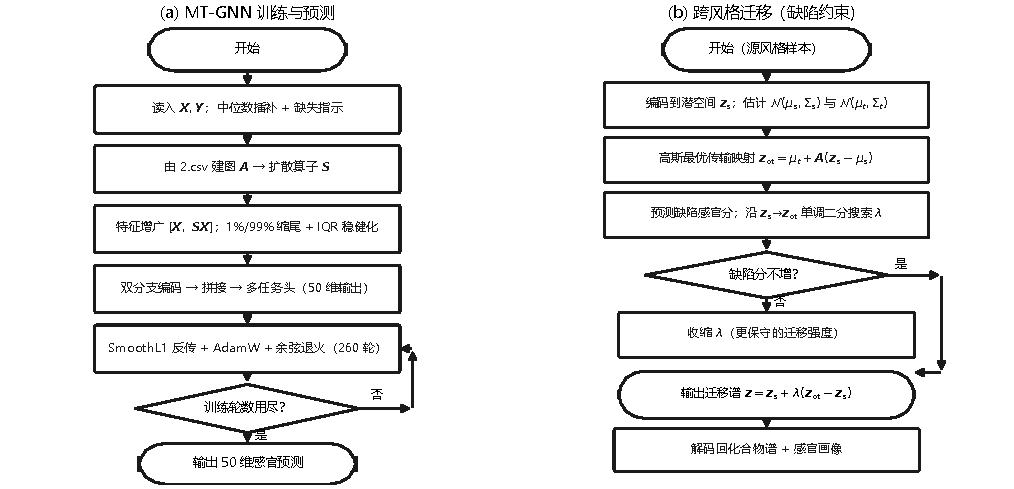
\includegraphics[width=\figw]{images/fig15_algorithm.pdf}
\caption{算法步骤图：(a) MT-GNN 的双分支编码与多任务训练回路；
(b) 跨风格迁移中“最优传输 + 单调二分投影”的缺陷约束流程}
\label{fig:algorithm}
\end{figure}

\section{支撑材料与源程序清单}

\subsection{提交文件清单}

全部源代码、中间结果与图件按下列结构组织，运行 \texttt{python src/01\_audit.py}
至 \texttt{src/08\_fig\_q3.py} 即可从原始附件完整复现本文全部数字与图件。

\begin{table}[H]
\centering
\caption{支撑材料文件清单}
\label{tab:files}
\small
\begin{fittable}
\begin{tabular}{@{}lll@{}}
\toprule
路径 & 功能 & 主要产物 \\
\midrule
\texttt{src/01\_audit.py} & 数据审计：对齐、底数、删失、0--6 标定 & \texttt{audit\_report.txt} \\
\texttt{src/common.py} & 共享模块：映射、元数据、OAV、社区发现 & --- \\
\texttt{src/02\_q1.py} & 问题一：十类模型横向比较 + 堆叠 + 区间 & \texttt{q1\_cv.json} \\
\texttt{src/03\_q2.py} & 问题二：共表达图 + 五路证据 + 稳定性 & \texttt{q2\_top3.csv} \\
\texttt{src/04\_q3.py} & 问题三：条件流 + 迁移 + 缺陷约束 & \texttt{q3\_summary.json} \\
\texttt{src/05\_fig\_data.py} & 图 1--3（审计与探索） & \texttt{latex/images/} \\
\texttt{src/05b\_fig\_schematic.py} & 图 0、图 15（路线与算法） & \texttt{latex/images/} \\
\texttt{src/06\_fig\_q1.py} & 图 4--7（问题一结果） & \texttt{latex/images/} \\
\texttt{src/07\_fig\_q2.py} & 图 8--10（问题二结果） & \texttt{latex/images/} \\
\texttt{src/08\_fig\_q3.py} & 图 11--14（问题三结果） & \texttt{latex/images/} \\
\texttt{output/} & 全部中间结果与交付表 & \texttt{q1\_scores\_06.csv} 等 \\
\texttt{latex/} & 论文源文件与图件（PDF 矢量） & \texttt{main.pdf} \\
\bottomrule
\end{tabular}
\end{fittable}
\end{table}

\subsection{核心程序：图扩散算子与多任务网络}

\begin{lstlisting}[language=Python,basicstyle=\ttfamily\scriptsize,
  frame=single,numbers=left,numberstyle=\tiny,xleftmargin=1.6em,
  breaklines=true,showstringspaces=false,
  commentstyle=\color{gray},keywordstyle=\color{black}\bfseries,
  stringstyle=\color{black}]
def build_graph(topk=8, alpha=0.35):
    """由 2.csv 相关矩阵构建共表达图与扩散算子 S。"""
    R, _, _, _ = C.corr_cc_aligned(COMP, META)      # 已对齐到 1.csv 列序
    W = np.abs(np.nan_to_num(R, nan=0.0))
    np.fill_diagonal(W, 0.0)
    k = min(topk, W.shape[0] - 1)
    idx = np.argpartition(-W, k, axis=1)[:, :k]     # 每行保留 top-k 强边
    M = np.zeros_like(W)
    for i in range(W.shape[0]):
        M[i, idx[i]] = W[i, idx[i]]
    M = np.maximum(M, M.T)                          # 对称化
    deg = M.sum(axis=1)
    dinv = np.where(deg > 0, 1.0 / np.sqrt(deg), 0.0)
    Ahat = (M * dinv[:, None]) * dinv[None, :]      # 归一化邻接
    return M, (1 - alpha) * np.eye(Ahat.shape[0]) + alpha * Ahat


class MTGNN:
    """双分支多任务网络：原始特征 + 图扩散特征，共享隐层、50 维输出。"""
    def fit(self, Xtr, Ytr):
        torch.manual_seed(self.seed)
        n, p = Xtr.shape
        k = Ytr.shape[1]
        self.p1 = p // 2                            # 前半为原始块，后半为扩散块
        self.mu = Ytr.mean(0); self.sd = Ytr.std(0) + 1e-8
        Yz = (Ytr - self.mu) / self.sd
        ...
        for ep in range(self.epochs):
            net.train()
            perm = torch.randperm(n)
            for i in range(0, n, bs):
                idx = perm[i:i + bs]
                opt.zero_grad()
                lossf(net(Xt[idx]), Yt[idx]).backward()
                opt.step()
            sch.step()
        self.net = net.eval()
        return self
\end{lstlisting}

\subsection{核心程序：高斯最优传输与缺陷约束投影}

\begin{lstlisting}[language=Python,basicstyle=\ttfamily\scriptsize,
  frame=single,numbers=left,numberstyle=\tiny,xleftmargin=1.6em,
  breaklines=true,showstringspaces=false,
  commentstyle=\color{gray},keywordstyle=\color{black}\bfseries,
  stringstyle=\color{black}]
def ot_map(mu_s, S_s, mu_t, S_t):
    """高斯 Bures-Wasserstein 最优传输：z' = mu_t + A (z - mu_s)。"""
    Ss_12 = sqrtm_psd(S_s)
    inner = sqrtm_psd(Ss_12 @ S_t @ Ss_12)
    A = np.linalg.pinv(Ss_12) @ inner @ np.linalg.pinv(Ss_12)
    return mu_t, A

# 沿 z_s -> z_ot 单调二分，取满足“缺陷感官分不增”的最远可行点
lam = np.ones(len(z_src))
base = defect_score(S_before)
bad = defect_score(S_after) > base
if bad.any():
    lo = np.zeros(bad.sum()); hi = np.ones(bad.sum())
    for _ in range(22):
        mid = (lo + hi) / 2
        Lz = Lsrc[bad] + mid[:, None] * (L_ot[bad] - Lsrc[bad])   # 化合物空间插值
Lz = enforce_defect_pareto(Lz, Lsrc[bad])                 # 缺陷列钳制到 [下界, 源值]
        ss = defect_score(predict_sensory_from_logx(decode(zz)))
        ok = ss <= base[bad]
        hi = np.where(ok, mid, hi); lo = np.where(ok, lo, mid)
    lam[bad] = hi
L_fin = enforce_defect_pareto(Lsrc + lam[:, None] * (L_ot - Lsrc), Lsrc)
\end{lstlisting}

\subsection{判定为原始浓度的 33 个化合物列}

\begin{table}[H]
\centering
\caption{经校准浓度表反证判定为“原始浓度”的 33 列（未做对数变换）}
\label{tab:rawall}
\scriptsize
\begin{fittable}
\begin{tabular}{@{}llll@{}}
\toprule
列名 & 类别 & 列名 & 类别 \\
\midrule
\texttt{X2.methyltetrahydrofuran.3.one} & 酮类 & \texttt{ethyl.butyrate} & 酯类 \\
\texttt{gamma.nonalactone} & 内酯类 & \texttt{ethyl.isobutyrate} & 酯类 \\
\texttt{X.E..beta.damascenone} & 萜烯类 & \texttt{ethyl.nicotinate} & 酯类 \\
\texttt{X3.methylbutanal} & 醛类 & \texttt{ethyl.pentanoate} & 酯类 \\
\texttt{X2.3.butanedione} & 酮类 & \texttt{eugenol} & 酚类 \\
\texttt{E.caryophyllene} & 萜烯类 & \texttt{furfural} & 呋喃类 \\
\texttt{linalool} & 萜烯类 & \texttt{geraniol} & 萜烯类 \\
\texttt{X.E..2.nonenal} & 醛类 & \texttt{hexyl.acetate} & 酯类 \\
\texttt{citronellol} & 萜烯类 & \texttt{methylpyrazine} & 吡嗪类 \\
\texttt{n.hexanol} & 醇类 & \texttt{n.hexanol} & 醇类 \\
\texttt{X1.alpha.terpineol} & 萜烯类 & \texttt{phenylacetaldehyde} & 醛类 \\
\texttt{alpha.humulene} & 萜烯类 & \texttt{styrene} & 其他 \\
\texttt{benzaldehyde} & 醛类 & \texttt{X2.ethyl.3.methylpyrazine} & 吡嗪类 \\
\texttt{benzyl.alcohol} & 醇类 & \texttt{X3Z.hexenol} & 醇类 \\
\texttt{diethyl.succinate} & 酯类 & \texttt{X5.methylfurfural} & 呋喃类 \\
\texttt{amyl.acetate} & 酯类 & \texttt{Z.nerolidol} & 萜烯类 \\
\texttt{X.E..beta.ocimene} & 萜烯类 & & \\
\texttt{X.E.E..2.4.decadienal} & 醛类 & & \\
\bottomrule
\end{tabular}
\end{fittable}
\end{table}

\subsection{人工智能工具使用说明}

依照竞赛《人工智能工具及输出使用规定》，本文对 AI 工具的使用范围作如下如实说明。

\begin{table}[H]
\centering
\caption{人工智能工具使用留痕}
\label{tab:ai}
\small
\begin{fittable}
\begin{tabular}{@{}p{0.16\textwidth}p{0.30\textwidth}p{0.44\textwidth}@{}}
\toprule
环节 & 使用的 AI 工具 & 参与内容与核查方式 \\
\midrule
数据审计 & DeepSeek-V4.1-Flash & 辅助编写审计脚本；所有判定（底数 10、
$33$ 列原始浓度、$102$ 列封底）均由脚本对附件数据实算给出，可复现 \\
模型构建 & DeepSeek-V4.1-Flash & 辅助实现模型代码与超参数网格；模型结构、
评价协议与结论由作者确定并交叉验证 \\
论文写作 & DeepSeek-V4.1-Flash & 辅助语言润色与 LaTeX 排版；技术判断、
结果解读与创新点归属作者 \\
\bottomrule
\end{tabular}
\end{fittable}
\end{table}

\textbf{留痕声明}：本文全部源程序文件开头的注释块均标注了 AI 辅助工具的名称
（DeepSeek-V4.1-Flash）、开发机构（深度求索）与版本年份；论文中所有模型公式均
给出可复核的推导过程或文献来源（见参考文献），不存在无推导、无引用且无法确认
来源的模型或公式。上述标注内容存在不被评阅认可的风险，特此说明。

\textbf{工具版本}：DeepSeek-V4.1-Flash，开发机构：深度求索（DeepSeek），
使用年份：2026 年。
